% -*- mode: tex; fill-column: 115; -*-

\documentclass[a4paper, twoside]{article}
\setcounter{secnumdepth}{5}
\setcounter{tocdepth}{5}
\usepackage[english]{babel}
\usepackage{textcomp}
\usepackage{amsmath,amsthm,amsfonts,amssymb,epsfig}
\usepackage{array}
\usepackage{datetime}
\usepackage{lipsum}% http://ctan.org/pkg/lipsum
\usepackage[left=1.1in,top=1in,right=1.1in]{geometry}% http://ctan.org/pkg/geometry
\usepackage{listings}% http://ctan.org/pkg/listings
\usepackage{spverbatim}
\usepackage{hyperref}
\usepackage{microtype}
\hypersetup{colorlinks=true, urlcolor=black, linkcolor=black}
\usepackage{graphicx}
\graphicspath{ {images/} }
\usepackage{parskip}
\usepackage{titlesec} %used for diminishing heading sizes
\usepackage[square, sort, comma, numbers]{natbib} %%uses titles for cited references
\usepackage[fit]{truncate}
\usepackage{fancyhdr}
\pagestyle{fancy}
\fancyhead{}
\fancyhead[RO, RE]{\thepage}
\fancyhead[LO, LE]{\rightmark}
\renewcommand{\sectionmark}[1]{\markboth{}{\textsc{\thesection~#1}}}
\fancyfoot[C]{}%hide footer
\usepackage{xcolor} 
\usepackage[scaled=1]{couriers}

\xdefinecolor{gray}{rgb}{0.6,0.6,0.6} 

% produced as part of ./gradlew booklets
\input{generated_buildinfo.tex}

\defcitealias{glmnet}{Regularization Paths for Generalized Linear Models via Coordinate Descent by Friedman et. al}
\defcitealias{strong}{Strong Rules for Discarding Predictors in Lasso-type Problems by Bien et. al}
\defcitealias{admm}{Distributed Optimization and Statistical Learning via the Alternating Direction Method of Multipliers by Boyd et. al}
\defcitealias{prox}{Proximal Algorithms by Boyd et. al}


\titleformat*{\section}{\LARGE\bfseries\sffamily}
\titleformat*{\subsection}{\Large\bfseries\sffamily}
\titleformat*{\subsubsection}{\large\bfseries\sffamily}
\titleformat*{\paragraph}{\large\bfseries\sffamily}
\titleformat*{\subparagraph}{\large\bfseries\sffamily}
\renewcommand{\familydefault}{\sfdefault} %sans-serif font



\begin{document}


%----------------------------------------------------------------------
% Definition for "lstlisting" blocks
%----------------------------------------------------------------------
% --- USAGE ---
%
% \begin{lstlisting}[style=R}
% ...
% \end{lstlisting}
%
% % \begin{lstlisting}[style=output}
% ...
% \end{lstlisting}
%----------------------------------------------------------------------

% By default, make listings all black so it's easy to spot the ones that aren't set to a style.
% This is just a debugging technique.
\lstset{backgroundcolor=\color{black}}

% Define scala language first
% ``define'' Scala
\lstdefinelanguage{scala}{
  morekeywords={abstract,case,catch,class,def,%
    do,else,extends,false,final,finally,%
    for,if,implicit,import,match,mixin,%
    new,null,object,override,package,%
    private,protected,requires,return,sealed,%
    super,this,throw,trait,true,try,%
    type,val,var,while,with,yield},
  otherkeywords={=>,<-,<\%,<:,>:,\#,@},
  sensitive=true,
  morecomment=[l]{//},
  morecomment=[n]{/*}{*/},
  morestring=[b]``,
  morestring=[b]',
  morestring=[b]''``
}

\lstdefinestyle{R}{
  language=R,
  frame=single,
  breaklines,
  basicstyle=\ttfamily,
  commentstyle=\textbf,% comment style
  keywordstyle=\ttfamily,
  numbers=left,% display line numbers on the left side 
  numberstyle=\scriptsize,% use small line numbers 
  numbersep=10pt,% space between line numbers and code
  backgroundcolor=\color{white}, 
  showstringspaces=false % don't show spaces as weird char.
}

\lstdefinestyle{python}{
  language=python,
  frame=single,
  breaklines,
  basicstyle=\ttfamily,
  commentstyle=\textsl,% comment style
  keywordstyle=\ttfamily,
  numbers=left,% display line numbers on the left side 
  numberstyle=\scriptsize,% use small line numbers 
  numbersep=10pt,% space between line numbers and code
  backgroundcolor=\color{white}, 
  showstringspaces=false %don't show spaces as weird char.
}

\lstdefinestyle{Scala}{
  language=scala,
  frame=single,
  breaklines,
  basicstyle=\ttfamily,
  commentstyle=\textsl,% comment style
  keywordstyle=\ttfamily,
  numbers=left,% display line numbers on the left side 
  numberstyle=\scriptsize,% use small line numbers 
  numbersep=10pt,% space between line numbers and code
  backgroundcolor=\color{white}, 
  showstringspaces=false % don't show spaces as weird char.
}

\lstdefinestyle{Bash}{
  language=bash,
  frame=single,
  breaklines,
  basicstyle=\ttfamily,
  commentstyle=\textsl,% comment style
  keywordstyle=\ttfamily,
  numbers=left,% display line numbers on the left side 
  numberstyle=\scriptsize,% use small line numbers 
  numbersep=10pt,% space between line numbers and code
  backgroundcolor=\color{white}, 
  showstringspaces=false % don't show spaces as weird char.
}


\definecolor{mygray}{rgb}{0.92,0.92,0.92}

\lstdefinestyle{output}{
  frame=single,
  breaklines,
  basicstyle=\ttfamily,
  numbers=left,% display line numbers on the left side 
  numberstyle=\scriptsize,% use small line numbers 
  numbersep=10pt,% space between line numbers and code
  backgroundcolor=\color{mygray}, 
  showstringspaces=false %don't show spaces as weird char.
}

\newcommand{\waterExampleInR} {
\textbf{Example in R} \\
}

\newcommand{\waterExampleInPython} {
\textbf{Example in Python} \\
}


\thispagestyle{empty} %removes page number

\begin{center}
\textsc{\Large\bf{Generalized Linear Modeling with H2O}}
\\
\bigskip
\textsc{\small{Tomas Nykodym \hspace{20pt} Ariel Rao \hspace{20pt} Amy Wang \hspace{20pt} Tom Kraljevic \hspace{20pt} Jessica Lanford}}
\\
\bigskip
\line(1,0){250}  %inserts  horizontal line

{\url{http://h2o.gitbooks.io/glm-with-h2o/}}

\bigskip
August 2015: Third Edition 

(Built for H2O version \waterVersion)
\\%add front page image here? (wavy lines)
\bigskip
\end{center}

{\raggedright\vfill\ 

Generalized Linear Modeling with H2O\\
  by Tomas Nykodym, Ariel Rao, Amy Wang, Tom Kraljevic, \&\ Jessica Lanford \\
\bigskip
  Published by H2O.ai, Inc. \\
2307 Leghorn St. \\
Mountain View, CA 94043\\
\bigskip
\textcopyright 2015 H2O.ai, Inc. All Rights Reserved. 
\bigskip

August 2015: Third Edition
\bigskip

Photos by \textcopyright H2O.ai, Inc.
\bigskip

While every precaution has been taken in the\\
preparation of this book, the publisher and\\
authors assume no responsibility for errors or\\
omissions, or for damages resulting from the\\
use of the information contained herein.\\
\bigskip
Printed in the United States of America. 
}

\newpage

\tableofcontents

%----------------------------------------------------------------------
%----------------------------------------------------------------------

\newpage

\section{Introduction}
This document introduces the reader to Generalized Linear Modeling with H2O.  Examples are written in R and python.
The reader is walked through the installation of H2O, basic GLM concepts, building GLM models in H2O, how to
interpret model output, how to make predictions, and various implementation details.

%----------------------------------------------------------------------
%----------------------------------------------------------------------

\section{What is H2O?}
\Urlmuskip=0mu plus 1mu\relax %needed to make long URLs break nicely


H2O is fast, scalable, open-source machine learning and deep learning for smarter applications. With H2O, enterprises like PayPal, Nielsen Catalina, Cisco, and others can use all their data without sampling to get accurate predictions faster. Advanced algorithms such as deep learning, boosting, and bagging ensembles are built-in to help application designers create smarter applications through elegant APIs. Some of our initial customers have built powerful domain-specific predictive engines for recommendations, customer churn, propensity to buy, dynamic pricing, and fraud detection for the insurance, healthcare, telecommunications, ad tech, retail, and payment systems industries.

Using in-memory compression, H2O handles billions of data rows in-memory, even with a small cluster. To make it easier for non-engineers to create complete analytic workflows, H2O's platform includes interfaces for R, Python, Scala, Java, JSON, and CoffeeScript/JavaScript, as well as a built-in  web interface, Flow. H2O was built alongside (and on top of) Hadoop and Spark Clusters and typically deploys within minutes.

H2O includes many common machine learning algorithms, such as generalized linear modeling (linear regression, logistic regression, etc.), Na\"{i}ve Bayes, principal components analysis, time series, k-means clustering, and others. H2O also implements best-in-class algorithms at scale, such as distributed random forest, gradient boosting and deep learning. Customers can build thousands of models and compare the results to get the best predictions.

H2O is nurturing a grassroots movement of physicists, mathematicians, and computer scientists to herald the new wave of discovery with data science by collaborating closely with academic researchers and Industrial data scientists. Stanford university giants Stephen Boyd, Trevor Hastie, Rob Tibshirani advise the H2O team on building scalable machine learning algorithms. With hundreds of meetups over the past three years, H2O has become a word-of-mouth phenomenon, growing amongst the data community by a hundred-fold, and is now used by 30,000+ users and is deployed using R, Python, Hadoop, and Spark in 2000+ corporations.

\textbf{Try it out}

\begin{itemize}
\item  Download H2O directly at \mbox{\url{http://h2o.ai/download}}.
\item Install H2O's R package from CRAN at {\url{https://cran.r-project.org/web/packages/h2o/}}. 
\item Install the Python package from PyPI at {\url{https://pypi.python.org/pypi/h2o/}}.

\end{itemize}



\textbf{Join the community}
\begin{itemize}
\item  To learn about our meetups, training sessions, hackathons, and product updates, visit {\url{http://h2o.ai}}. 
\item Visit the open source community forum at {\url{https://groups.google.com/d/forum/h2ostream}}.
\item Join the chat at {\url{https://gitter.im/h2oai/h2o-3}}.
\end{itemize}





%----------------------------------------------------------------------
%----------------------------------------------------------------------

\newpage

\section{Installation} 
\Urlmuskip=0mu plus 1mu\relax %needed to make long URLs break nicely


The easiest way to directly install H2O is  via an R or Python package.

({\bf{Note}}: The examples in this document were created with H2O version \waterVersion.)

\subsection{Installation in R}

To load a recent H2O package from CRAN, run:

\begin{lstlisting}[style=R]
install.packages("h2o")
\end{lstlisting}

{\bf{Note}}: The version of H2O in CRAN is often one release behind the current version.

For the latest recommended version, download the
latest stable H2O-3 build from the H2O download page:

\begin{enumerate}
\item Go to {\url{http://h2o.ai/download}}.
\item Choose the latest stable H2O-3 build.
\item Click the ``Install in R'' tab.
\item Copy and paste the commands into your R session.
\end{enumerate}

\bigskip
After H2O is installed on your system, verify the installation:

\begin{lstlisting}[style=R]
library(h2o)

#Start H2O on your local machine using all available cores.
#By default, CRAN policies limit use to only 2 cores.
h2o.init(nthreads = -1)

#Get help
?h2o.glm
?h2o.gbm

#Show a demo
demo(h2o.glm)
demo(h2o.gbm)
\end{lstlisting}

\subsection{Installation in Python}

To load a recent H2O package from PyPI, run:

\begin{lstlisting}[style=python]
pip install h2o
\end{lstlisting}

To download the
latest stable H2O-3 build from the H2O download page:

\begin{enumerate}
\item Go to {\url{http://h2o.ai/download}}.
\item Choose the latest stable H2O-3 build.
\item Click the ``Install in Python'' tab.
\item Copy and paste the commands into your Python session.
\end{enumerate}

\bigskip
After H2O is installed, verify the installation:

\begin{lstlisting}[style=python]
import h2o

# Start H2O on your local machine
h2o.init()

# Get help
help(h2o.glm)
help(h2o.gbm)

# Show a demo
h2o.demo("glm")
h2o.demo("gbm")

\end{lstlisting}

\subsection{Pointing to a Different H2O Cluster}

The instructions in the previous sections create a one-node H2O cluster on your local machine. 

To connect to an established H2O cluster (in a multi-node Hadoop environment, for example) specify the IP address and port number for the established cluster using the \texttt{ip} and \texttt{port} parameters in the \texttt{h2o.init()} command.  The syntax for this function is identical for R and Python:
\medskip  

\begin{lstlisting}[style=R]
h2o.init(ip = "123.45.67.89", port = 54321)
\end{lstlisting}

%if it's the same, only one is needed



\subsection{Example code}

R code for the examples in this document are available here:

\url{https://github.com/h2oai/h2o-3/blob/master/h2o-docs/src/booklets/v2_2015/source/GLM_Vignette.R}

Python code for the examples in this document can be found here:

\url{https://github.com/h2oai/h2o-3/blob/master/h2o-docs/src/booklets/v2_2015/source/GLM_Vignette.py}

The document source itself can be found here:

\url{https://github.com/h2oai/h2o-3/blob/master/h2o-docs/src/booklets/v2_2015/source/GLM_Vignette.tex}

%----------------------------------------------------------------------
%----------------------------------------------------------------------

\section{GLM Concepts}
Generalized linear models (GLM) are the workhorse for most predictive analysis use cases. GLM scales well to large datasets, is based on a solid statistical background, and can be used for both regression and classification. It
is a generalization of linear models, allowing for modeling of data with exponential distributions and for
categorical data (classification). GLM models are fitted by solving the maximum likelihood optimization problem.

Generalized linear models are generalizations of linear regression models. Linear regression models the dependency
of response $y$ on a vector of predictors $x$ ($y \sim x^T \beta + \beta_0$). The models are built with the assumptions
that y has a Gaussian distribution with a variance of $\sigma^2$ and the mean is a linear function of x with an
offset of some constant $\beta_0$, i.e. $ y = \mathcal{N}(x^T \beta + \beta_0 , \sigma^2) $. These assumptions can
be overly restrictive for real-world data that do not necessarily have a Gaussian distribution.

GLM generalizes linear regression in the following ways: 

\begin{itemize} 
\item adding a non-linear link function that transforms the expectation of response variable, so that $link(y) \sim x^T \beta + \beta_0$.
\item allowing variance to depend on the predicted value by specifying the conditional distribution of the response variable or the family argument.
\end{itemize}

This generalization allows us to use GLM on problems such as binary classification (also known as logistic regression).

\subsection{GLM in H2O}
H2O's GLM algorithm fits the generalized linear model with elastic net penalties. The model fitting computation is
distributed, extremely fast, and scales extremely well for models with a limited number ($\mathtt{\sim}$ low
thousands) of predictors with non-zero coefficients. The algorithm can compute models for a single value of a
penalty argument or the full regularization path, similar to the glmnet package for R (refer
to \citetalias{glmnet}).  H2O's GLM fits the model by solving following problem:

\[ \min\limits_{\beta}\ (\ Classic GLM  + Regularization Penalty \ )\]

which is equivalent to:

\[ \min\limits_{\beta}\ (\ {{1\over{N}} log\_likelihood(family,\beta)  + \lambda (\alpha \| \beta \|_1} + {1- \alpha \over 2} \| \beta \|_2^2) \ )\]

\bigskip
The elastic net parameter $\alpha$ controls the penalty distribution between L1 (Lasso) and L2 (Ridge Regression)
penalties. The range is any value between 0 and 1. When $\alpha$ = 0, we have no L1 penalty and the problem becomes
ridge regression. If $\alpha$ = 1, there is no L2 penalty and we have Lasso.

The main advantage of an L1 penalty is that with sufficiently high $\lambda$, it produces a sparse solution; the
L2-only penalty does not reduce coefficients to exactly 0. The two penalties also differ in the case of correlated
predictors. The L2 penalty shrinks coefficients for correlated columns towards each other, while the L1 penalty
will pick one and drive the others to zero. Using the elastic net argument $\alpha$, you can combine these two
behaviors. It is also useful to always add a small L2 penalty to increase numerical stability.

Similarly to the methods discussed in \citetalias{glmnet}, H2O can compute the full regularization path, starting
from a null-model (maximum penalty) down to a minimally-penalized model. To improve the efficiency of this search, 
H2O employs strong-rules as described in \citetalias{strong} to filter out inactive coefficients (coefficients pushed
to zero by penalty). Computing the full regularization path is useful because it gives more insight about the
importance of individual coefficients and quality of the model while allowing selection of the optimal amount of
penalization for the given problem and data.

\subsection{Model fitting}
GLM models are fitted by maximizing the likelihood. For the Gaussian family, maximum likelihood is simply the
minimal mean squared error, which has an analytical solution and can be solved with a standard method of least squares. For all other families, the maximum likelihood problem has no analytical solution so we must use an iterative method such
as IRLSM, Newton method, gradient descent, or L-BFGS.

\subsection{Model validation}
Evaluating the quality of the model is a critical part of the data-modeling and scoring process. There are several
standard ways to evaluate the quality of the fitted GLM model; the most common method is to use the resulting
deviance. Deviance is calculated by comparing the log likelihood of the fitted model with the log likelihood of the
saturated model (or theoretically perfect model).

\[ deviance = 2({ln(L_{s})} - {ln(L_{m})}) \]

Another metric frequently used for model selection is the Akaike information criterion (AIC). The AIC measures the
relative quality of a statistical model for a given set of data obtained by calculating the information loss after
replacing the original data with the model itself. Unlike deviance, which would assign a perfect value for the
saturated model and measures the absolute quality of the fit with a comparison against the null-hypothesis, AIC
takes into account the complexity of the given model. AIC is defined as follows:

\[ aic = 2(k - ln(L_{m}))\]

where $k$ is the number of model parameters and $ln(L_{m})$ is the log likelihood of the fitted model over the data.

\subsection{Regularization} \label{regularization}
We introduce penalties to the model building process to avoid over-fitting, reduce variance of the prediction
error, and handle correlated predictors. There are two common penalized linear models: ridge regression and
Lasso (least absolute shrinkage and selection operator). Ridge regression provides greater numerical stability and is easier and faster to compute. In comparison, Lasso leads to a sparse solution, which is advantageous in many situations, as it can be used for feature selection and to produce models with fewer parameters. When encountering highly correlated columns, the L2 penalty tends to push all of the coefficients towards each other, while the L1 penalty will pick one and remove the others to produce 0 coefficients.

\subsubsection{Lasso and Ridge regression}

Lasso represents the L1 penalty and is an alternative regularized least squares method that uses the constraint
$||B||_1$. The main difference between Lasso and
ridge regression is that as the penalty for ridge regression increases, the parameters are reduced to non-zero
values. With Lasso, if the penalty is increased, the parameters can be reduced to zero values. Since reducing
parameters to zero removes them from the model, the Lasso method only relies on the relevant data (discards the noise). Ridge regression never removes any predictors.

\subsubsection{Elastic net penalty}

H2O supports elastic net regularization, which is a combination of L1 and L2 penalties and is parametrized by \texttt{alpha} and \texttt{lambda} arguments
(similar to \citetalias{glmnet}).

The \texttt{alpha} argument controls the elastic net penalty distribution to L1 and L2 norms. It can have any value
in the [0,1] range (inclusive) or a vector of values (which triggers grid search). If \texttt{alpha = 0}, the result
is \textbf{Ridge Regression}, while if \texttt{alpha = 1} the result is \textbf{LASSO}.

The \texttt{lambda} argument controls the penalty strength; the range is any positive value or a vector of values
(which triggers grid search).

\textbf{Note:} Lambda values are capped at $\lambda_{max}$, which is the smallest $\lambda$ s.t. the solution is
empty model (all zeros except for intercept). %%this needs to be clarified - it doesn't really make sense to me. 

The combination of L1 and L2 penalties is beneficial, since L1 gives sparsity while L2 gives
stability and encourages the grouping effect (where a group of correlated variables tends to be dropped or added
into the model all at once). One possible use of the $\alpha$ argument is for Lasso with very little L2 penalty
($\alpha$ almost 1) to stabilize the computation and improve convergence speed.

A model-fitting problem with an elastic net penalty becomes:

\[ \min\limits_{\beta,\beta_0}\ {{1\over{N}} ln(L(family,\beta,\beta_0))  + \lambda (\alpha \| \beta \|_1}  + {1- \alpha \over 2} \| \beta \|_2^2) \]

\subsection{GLM model families}
The following subsection describes the GLM families supported in H2O. 

\subsubsection{Linear regression (Gaussian family)}
Linear regression refers to the Gaussian family model. It is the simplest example of GLM, but it has many uses and
several advantages over the other families, such as faster and more stable computation.

It models the dependency as a purely linear function (with link = identity):
\[ \hat{y} = x^T\beta + \beta_0\]

The model is fitted by solving the least squares problem (maximum likelihood for Gaussian family):

\[ \min\limits_{\beta,\beta_0} { {1 \over 2N}\sum\limits_{i=1}\limits^{N}(x_i^{T}\beta  + \beta_0- y_i)^T (x_i^{T}\beta + \beta_0 - y_i)  + \lambda (\alpha \|\beta \|_1 + {1-\alpha \over 2}) \| \beta \|_2^2} \]

Deviance is simply the sum of squared errors:
\[ D = \sum\limits_{i=1}\limits^{N}{(y_i - \hat{y}_i)^2} \]

\waterExampleInR

Included in the H2O package is a prostate cancer data set. The data was collected by Dr. Donn Young at Ohio State
University Comprehensive Cancer Center for a study of patients with varying degrees of prostate cancer. The
following example illustrates how to build a model to predict the volume (VOL) of tumors obtained from ultrasounds
based on features such as age and race.
\bigskip
\lstinputlisting[style=R]{glm/glm_gaussian_example.R}

\waterExampleInPython
\lstinputlisting[style=python]{glm/glm_gaussian_example.py}

\subsubsection{Logistic regression (Binomial family)}
Logistic regression can be used for a binary classification problem where the response is categorical with two
levels. It models dependency as $Pr(y = 1|x)$. The canonical link for binomial family is logit (log of the odds)
and its inverse is a logistic function that takes any real number on the input and projects it onto the 0,1 range
(s-curve).  The s-curve is shown below:

\begin{figure}[h]
\centering
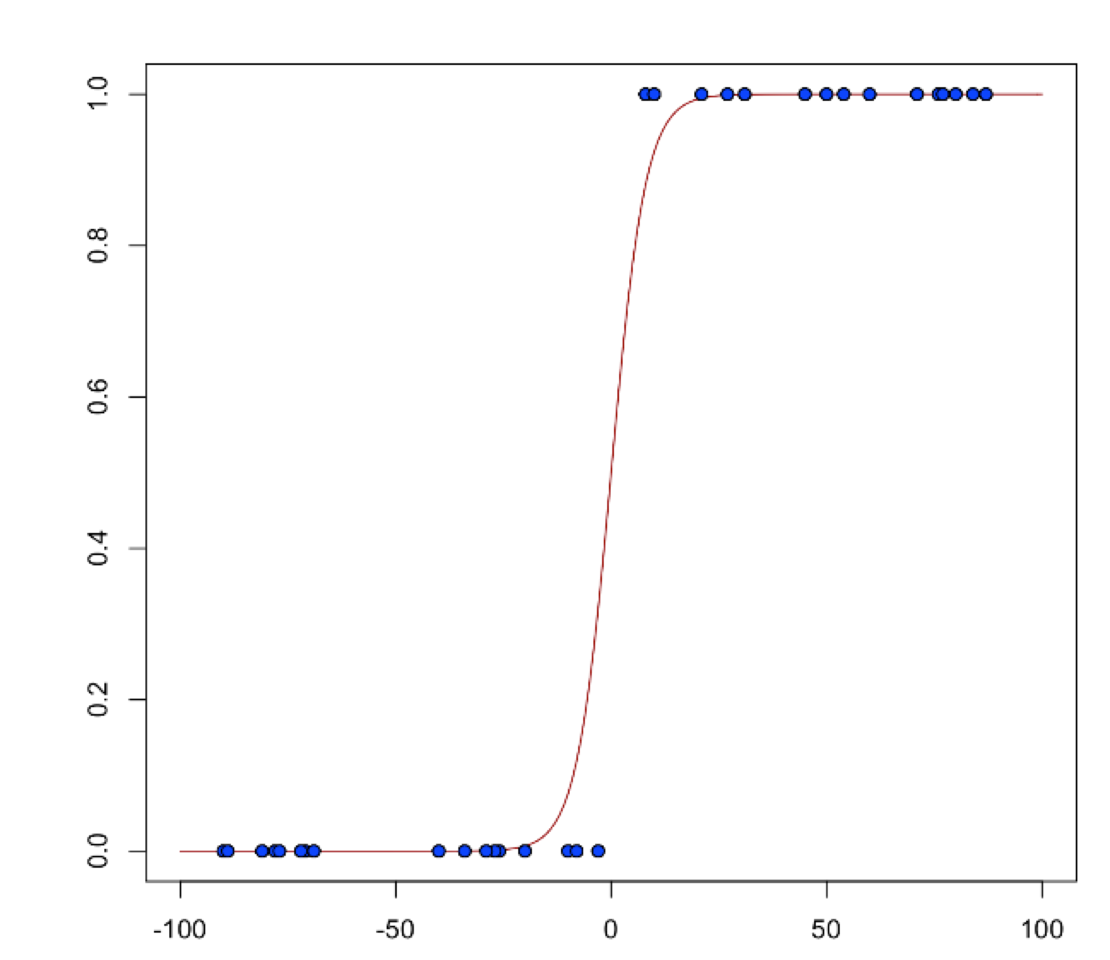
\includegraphics[scale=0.5]{images/scurve.png}
\end{figure}

\[ \hat{y} = Pr(y = 1|x) = {e^{x^T\beta + \beta_0} \over 1 + e^{x^T \beta + \beta_0} } \]

or alternatively:

\[log {\hat{y} \over 1- \hat{y}} = log{Pr(y=1|x) \over Pr(y=0|x)} = x^T \beta + \beta_0\]

The model is fitted by solving:
\[  \min\limits_{\beta,\beta_0} { {1 \over N}\sum\limits_{i=1}\limits^{N}(y_i (x_i^{T}\beta  + \beta_0) - log (1 + e^{x_i^{T}\beta  + \beta_0} )  + \lambda (\alpha \|\beta \|_1 + {1-\alpha \over 2}) \| \beta \|_2^2} \]

Deviance is -2 log likelihood:
\[D = -2\sum\limits_{i=1}\limits^{N}{(y log(\hat{y}) + (1 - y)log(1-\hat{y})  )}\]

\waterExampleInR

Using the prostate data set, this example builds a binomial model that classifies incidence of penetration of the prostatic
capsule (CAPSULE). Confirm the entries in the CAPSULE column are binary using the \texttt{h2o.table()}
function. Change the regression by changing the family to binomial.

\lstinputlisting[style=R]{glm/glm_binomial_example.R}

\waterExampleInPython
\lstinputlisting[style=python]{glm/glm_binomial_example.py}

\subsubsection{Poisson models}
Poisson regression is generally used in cases where the response represents counts and we assume errors have a
Poisson distribution. In general, it can be applied to any data where the response is non-negative.

When building a Poisson model, we usually model dependency of the mean on the log scale, i.e. canonical link is log
and prediction is:

\[\hat{y} = e^{x^T\beta + \beta_0}\]

The model is fitted by solving:

\[  \min\limits_{\beta,\beta_0} { {1 \over N}\sum\limits_{i=1}\limits^{N}(y_i (x_i^{T}\beta  + \beta_0) - e^{x_i^{T}\beta  + \beta_0})  + \lambda (\alpha \|\beta \|_1 + {1-\alpha \over 2}) \| \beta \|_2^2} \]

Deviance is:

\[D = -2\sum\limits_{i=1}\limits^{N}{(y log(\hat{y}) - y - \hat{y}}\]

\waterExampleInR
\\
This example loads the Insurance data from the MASS library, imports it into H2O, and runs a Poisson model that predicts the number of claims (Claims) based on the district of the policy holder (District), their age (Age), and the type of car they
own (Group).
\bigskip
\lstinputlisting[style=R]{glm/glm_poisson_example.R}

\waterExampleInPython
\lstinputlisting[style=python]{glm/glm_poisson_example.py}

\subsubsection{Gamma models}
The gamma distribution is useful for modeling a positive continuous response variable, where the conditional
variance of the response grows with its mean but the coefficient of variation of the response $\sigma^2(x)/μ(x)$ is
constant for all $x$, i.e., it has a constant coefficient of variation. It is usually used with inverse or log link, where inverse is the canonical link.

The model is fitted by solving:

\[  \min\limits_{\beta,\beta_0} { {1 \over N}\sum\limits_{i=1}\limits^{N}{y_i \over (x_i^{T}\beta  + \beta_0)} - log({x_i^{T}\beta  + \beta_0})  + \lambda (\alpha \|\beta \|_1 + {1-\alpha \over 2}) \| \beta \|_2^2} \]

Deviance is:

\[D = -2\sum\limits_{i=1}\limits^{N}{log({y_i \over \hat{y}_i}) - {y_i - \hat{y}_i \over\hat{y}_i }}\]

\waterExampleInR
\\
To change the link function from the default inverse function to the log link function, modify the \texttt{link}
argument.
\bigskip
\lstinputlisting[style=R]{glm/glm_gamma_example.R}

\waterExampleInPython
\lstinputlisting[style=python]{glm/glm_gamma_example.py}

\subsubsection{Tweedie models}

Tweedie models are a class of distributiions which include Gamma, Normal, Poisson and their combination. It is especially usefull for modelling of variables which have 0s combined with continuous non-zero values (e.g. Gamma distribution).

Tweedie is parametrized by variance power p which can be one of the following:

\begin{itemize}
\item  0	Normal
\item  1	Poisson
\item (1, 2)	Compound Poisson, non-negative with mass at zero
\item 2	Gamma
\item 3	Inverse-Gaussian
\item $>$ 2	Stable, with support on the positive reals
\end{itemize}


TODO fit in likelihood 

Deviance for variance p ($p != 1$ and $p != 2$) is :
\[
D = -2\sum\limits_{i=1}\limits^{N}{ y_i  (y_i^{1-p} - \hat{y_i}^{1-p}) - {(y^{2 - p} - \hat{y}^{2 - p})\over(2 - p)}}
\]

\waterExampleInR
\lstinputlisting[style=R]{glm/glm_tweedie_example.R}

\waterExampleInPython
\lstinputlisting[style=python]{glm/glm_tweedie_example.py}

%----------------------------------------------------------------------
%----------------------------------------------------------------------

\section{Building GLM Models in H2O}

H2O's GLM implementation presents a high-performance distributed algorithm that scales linearly with the number
of rows and works extremely well for datasets with a limited number of active predictors.

\subsection{Classification vs. regression}

GLM can produce two categories of models: classification (binary classification only) and regression.  Binary
classification in GLM is also called logistic regression.

The data type of the response column determines the model category.  If the response data type is a categorical
(also called a factor or an enum) then a classification model is created.  If the response column data type is
numeric (either integer or real), then a regression model is created.

The following examples show how to coerce the data type of a column to a factor.

\bigskip
\waterExampleInR
\lstinputlisting[style=R]{glm/coerce_column_to_factor.R}

\waterExampleInPython
\lstinputlisting[style=python]{glm/coerce_column_to_factor.py}

\subsection{Training and validation frames}

In this context, the word Frame refers to an H2OFrame, which is the fundamental method of data storage in H2O's distributed memory.

\texttt{training\_frame} refers to a frame containing a training dataset.  All predictors and the response (as
well as offset and weights, if specified) must be part of this frame.

\texttt{validation\_frame} refers to an optional frame containing a validation dataset.  If specified, this 
frame must have exactly the same columns as the training dataset.  Metrics are calculated on the validation dataset
for convenience.

If a validation dataset is not specified during training, there are functions that can calculate the same metrics after the model training is complete. %%would be helpful to provide examples or where users can find these functions. 

\subsection{Predictor and response variables}

Every model must specify its predictors and response.  Predictors and response are specified by the \texttt{x}
and \texttt{y} parameters.

\texttt{x} contains the list of column names or column indices referring to vectors from the training frame; it can
not contain periods.

\texttt{y} is a column name or index referring to a vector from the training frame.

\subsubsection{Categorical variables}

If the response column is categorical, then a classification model is created.  GLM only supports binomial
classification, so the response column may only have two levels.

Categorical predictor columns may have more than two levels.

We recommend letting GLM handle categorical columns itself, as it can take advantage of the categorical
column for better performance and memory utilization.

We strongly recommend avoidance of one-hot encoding categorical columns with many levels into many binary columns, as this is very inefficient.  This is especially true for Python users who are used to expanding their categorical variables
manually for other frameworks.

\subsection{Family and link}

Family and Link are both optional parameters. The default family is \texttt{Gaussian} and the default link is a
canonical link for the selected family. These are passed in as strings, e.g. \texttt{family=`gamma', link = `log'}.
While it is possible to select something other than a canonical link, doing so can lead to an unstable
computation. 

\subsection{Regularization parameters}

Refer to \nameref{regularization} above for a detailed explanation.

To get the best possible model, we need to find the optimal values of the regularization parameters $\alpha$ and
$\lambda$.  To find the optimal values, H2O provides grid search over $\alpha$ and a special form of grid search
called ``lambda search" over $\lambda$. The recommended way to find optimal regularization settings on H2O is to do
a grid search over a few $\alpha$ values with an automatic lambda search for each $\alpha$. Both are described
below in greater detail.

\subsubsection{alpha and lambda}

\texttt{alpha} controls the distribution between L1 (Lasso) and L2 (Ridge regression) penalties.  An \texttt{alpha} 
of 1.0 indicates only Lasso, and an \texttt{alpha} of 0.0 indicates only ridge.

\texttt{lambda} controls the amount of regularization applied.  For a \texttt{lambda} value of 0.0, no 
regularization is applied, and the \texttt{alpha} parameter is ignored.  The default value for \texttt{lambda} is
calculated by H2O using a heuristic based on the training data.  If you let H2O calculate \texttt{lambda}, you can
see the chosen value in the model output.

\subsubsection{Lambda Search}
Lambda search enables efficient and automatic search for optimal value of the \texttt{lambda} parameter. When lambda search is enabled, GLM will first fit a model with maximum regularization strength and then keep decreasing it until overfitting. The resulting model will be based on the best \texttt{lambda} value. When looking for sparse solution (\texttt{alpha} $>$ 0), lambda serach can also be used to efficiently handle very wide datasets as it can filter out inactive predictors (noise) and only build models for a small subset of predictors. Common use of lambda search is to run on a dataset with many predictors but limit the number of active predictors to relatively small value.  

Lambda search can be turned on by setting \texttt{lambda\_search} and can be further customized by following arguments:

\begin{itemize}
\item \texttt{alpha} - regularization distribution between L1 and L2
\item \texttt{validation\_frame} and\/or \texttt{n\_folds}:
The best lambda is selected based on performance on the cross-validation or validation or training data. If available, cross-validation performance takes preference. If no validation data is available, the best lambda is selected based on training data performance and is therefore guaranteed to always be the minimal lambda computed as GLM can not overfit on a trainign dataset.
 
\textbf{Note:} If running lambda search with validation dataset and no cross-validation, validation data set is used to select the lambda value, validation dataset is thus contaminated and performance should be evaluated on another independent dataset.


\item \texttt{lambda\_min\_ratio} and \texttt{nlambdas}: 

The sequence of $\lambda$-s is automatically generated as an exponentially decreasing sequence, going from $\lambda_{max}$,
the smallest $\lambda$ such that the solution is a model with all 0s, to $\lambda_{min} =
$ \textit{lambda\_min\_ratio} * $ \lambda_{max}$.

H2O computes $\lambda$-models sequentially and in decreasing order, warm-starting (using the previous solution as
the initial prediction) the model for $\lambda_k$ with the solution for $\lambda_{k-1}$. By warm-starting the
models, we get better performance: typically models for subsequent $\lambda$s are close to each other, so we need
only a few iterations per $\lambda$ (typically two or three). We also achieve greater numerical stability, since models
with a higher penalty are easier to compute, so we start with an easy problem and then keep making only small
changes to it.


\textbf{Note:} \texttt{nlambda} and \texttt{lambda\_min\_ratio} also specify the relative distance of any two
 lambdas in the sequence. This is important when applying recursive strong rules, which are only effective if the
neighboring lambdas are ``close" to each other. The default values are \texttt{nlambda} = 100 and $\lambda_{min}
= \lambda_{max} 1e^{-4}$, which gives us the ratio of 0.912.  For best results when using strong rules, keep the
ratio close to the default.

\item \texttt{max\_active\_predictors}: Limit the number of active predictors (the actual number of non-zero predictors in the model is going to be slightly lower), usefull when obtaining a sparse solution to avoid costly computation of models with too many predictors.

\end{itemize}


\subsection{Handling wide data and building sparse models}

H2O's GLM offers two different approaches to handling wide datasets:  L1 regularization and the L\_BFGS solver.

Quick recommendations:

\begin{itemize}
\item For a sparse solution (i.e. some predictors are dropped from the final model), use the IRLSM solver with 
      \texttt{alpha} greater than 0.0 (so you get at least some L1 penalty) and enable \texttt{lambda\_search}.

\item For a dense solution (i.e. all predictors are in the final model), use the L\_BFGS solver with
      \texttt{alpha} of 0 so there is no L1 penalty, only L2 penalty.
\item If not sure whether the solution should be sparse or dense, try both cases and pick the better one based on validation (cross-validation) data.      
\end{itemize}

\subsubsection{Solver selection}

The two solvers provided in H2O are Iterative Reweighted Least Squares Method (IRLSM) and Limited-memory Broyden-Fletcher-Goldfarb-Shanno (L\_BFGS).  IRLSM uses
a Gram Matrix approach underneath the hood, which is very efficient for tall and narrow datasets and when running lambda search with sparse solution.  For wider and dense
datasets (thousands of predictors and up), the L\_BFGS solver scales better.

For performance reasons, we recommend not using any L1 penalty when using the L\_BFGS solver, since
model building can be slower. It is often better to run lambda search with IRLSM solver instead.

\subsubsection{Stopping criteria}

When using L1 penalty with lambda search, you can specify the \texttt{max\_active\_predictors} parameter to stop
the search before it completes.  Models built at the beginning of the lambda search have higher lambda values, consider fewer predictors, and take less time to calculate the model.  Models built at the end of the lambda search have
lower lambda values, incorporate more predictors, and take a longer time to calculate the model. You can also set the \texttt{nlambdas} parameter for a lambda search to specify the number of models attempted across the search.

\bigskip
\waterExampleInR
\lstinputlisting[style=R]{glm/glm_stopping_criteria.R}

\waterExampleInPython
\lstinputlisting[style=python]{glm/glm_stopping_criteria.py}



\subsection{Advanced features}

H2O's GLM has several advanced features to help build better models.

\subsubsection{Standardizing data}

The \texttt{standardize} parameter, which is enabled by default, standardizes numeric columns to have zero mean and
unit variance.  This parameter must be enabled (using \texttt{standardize=TRUE}) to produce standardized coefficient magnitudes in the model output.

We recommend enabling standardization when using regularization (i.e. \texttt{lambda} is chosen by H2O or set by
the user to be greater than 0). Only advanced users should disable standardization.

\subsubsection{N-fold cross validation}

All validation values can be computed using either the training data set (the default option) or using N-fold
cross-validation (\texttt{nfolds $> 1$)}. When N-fold cross-validation is enabled, H2O randomly splits data into n
equally-sized parts, trains each of the n models on n-1 parts, and computes validation on the part that was not
used for training.

You can also specify the rows that are assigned to each fold using the \texttt{fold\_assignment}
or \texttt{fold\_column} parameters.

\bigskip
\waterExampleInR
\lstinputlisting[style=R]{glm/glm_cross_validation.R}



\subsubsection{Grid search over alpha}

Alpha search is not always needed and simply changing its value to 0.5 (or 0 or 1 if we only want Ridge or Lasso,
respectively) works in most cases. If $\alpha$ search is needed, specifying only a few values is typically sufficient. Alpha
search is invoked by supplying a list of values for $\alpha$ instead of a single value. H2O then produces one model
per $\alpha$ value. The grid search computation can be done in parallel (depending on the cluster resources) and it
is generally more efficient than computing different models separately from R.

Use caution when including $\alpha=0$ or $\alpha=1$ in the grid search. $\alpha=0$ will produce a dense solution
and it can be very slow (or even impossible) to compute in large $N$ situations. $\alpha=1$ has no L2 penalty, so
it is therefore less numerically stable and can be very slow as well due to slower convergence. In general, we recommend running with $alpha=1-\epsilon$ instead.

\waterExampleInR
\lstinputlisting[style=R]{glm/glm_grid_search_over_alpha.R}

\subsubsection{Grid search over lambda}

% While automatic lambda search is the preferred method, it is also possible to do a grid search over lambda values
% by passing in vector of lambdas and disabling the lambda-search option. The behavior will be identical to lambda
% search, except H2O will use a user-supplied list of lambdas instead (still capped at $\lambda_{max}$).

% \bigskip
% \waterExampleInR
% \lstinputlisting[style=R]{glm/glm_grid_search_over_lambda.R}

Grid search over lambda is a feature from H2O-2 that is not currently supported in H2O-3.  Instead, use the built-in lambda
search capability in GLM.

\subsubsection{Offsets}

\texttt{offset\_column} is an optional column name or index referring to a column in the training frame. This column specifies a prior known component to be included in the linear predictor during training. Offsets are per-row “bias values” that are used during model training. For Gaussian distributions, they can be seen as simple corrections to the response (y) column. Instead of learning to predict the response (y-row), the model learns to predict the (row) offset of the response column. For other distributions, the offset corrections are applied in the linearized space before applying the inverse link function to get the actual response values.  

\subsubsection{Row weights}

\texttt{weights\_column} is an optional column name or index referring to a column in the training frame. This column specifies on a per-row basis the weight of that row.  If no weight column is specified, a default value of 1 is used for each row. Weights are per-row observation weights. This is typically the number of times a row is repeated, but non-integer values are supported as well. During training, rows with higher weights matter more, due to the larger loss function pre-factor.

\subsubsection{Coefficient constraints}

Coefficient constraints allow you to set special conditions over the model coefficients. Currently supported
constraints are upper and lower bounds and the proximal operator interface, as described in \citetalias{prox}.

The constraints are specified as a frame with following vecs (matched by name; all vecs can be sparse):

\begin{itemize}
\item \texttt{names (mandatory)}  - coefficient names. 
\item \texttt{lower\_bounds (optional)} - coefficient lower bounds , must be $<= 0$
\item \texttt{upper\_bounds (optional)} - coefficient upper bounds , must be $>= 0$
\item \texttt{beta\_given (optional)} - specifies the given solution in proximal operator interface
\item \texttt{rho} (mandatory if \texttt{beta\_given} is specified, otherwise ignored) - specifies per-column L2 penalties on the distance from the given solution
\end{itemize}
 
\subsubsection{Proximal operators}

The proximal operator interface allows you to run the GLM with a proximal penalty on a distance from a specified
given solution. There are many potential uses: for example, it can be used as part of an ADMM consensus algorithm
to obtain a unified solution over separate H2O clouds, or in Bayesian regression approximation.

%----------------------------------------------------------------------
%----------------------------------------------------------------------

\section{GLM Model Output}

The following sections explain the output produced by logistic regression (i.e. binomial classification).

\bigskip
\waterExampleInR
\lstinputlisting[style=R]{glm/glm_model_output_10.R}

\begin{lstlisting}[style=output]
Model Details:
==============

H2OBinomialModel: glm
Model ID:  GLM_model_R_1439511782434_25 
GLM Model:
    family  link                                regularization number_of_predictors_total number_of_active_predictors number_of_iterations training_frame
1 binomial logit Elastic Net (alpha = 0.5, lambda = 4.674E-4 )                          4                           5                    5      subset_39

Coefficients:
      names coefficients standardized_coefficients
1 Intercept    -6.467393                 -0.414440
2       AGE    -0.021983                 -0.143745
3      RACE    -0.295770                 -0.093423
4       PSA     0.028551                  0.604644
5   GLEASON     1.156808                  1.298815

H2OBinomialMetrics: glm
** Reported on training data. **

MSE:  0.1735008
R^2:  0.2842015
LogLoss:  0.5151585
AUC:  0.806806
Gini:  0.6136121
Null Deviance:  403.9953
Residual Deviance:  307.0345
AIC:  317.0345

Confusion Matrix for F1-optimal threshold:
         0   1    Error     Rate
0      125  50 0.285714  =50/175
1       24  99 0.195122  =24/123
Totals 149 149 0.248322  =74/298

Maximum Metrics:
                      metric threshold    value idx
1                     max f1  0.301518 0.727941 147
2                     max f2  0.203412 0.809328 235
3               max f0point5  0.549771 0.712831  91
4               max accuracy  0.301518 0.751678 147
5              max precision  0.997990 1.000000   0
6           max absolute_MCC  0.301518 0.511199 147
7 max min_per_class_accuracy  0.415346 0.739837 134

H2OBinomialMetrics: glm
** Reported on validation data. **

MSE:  0.1981162
R^2:  0.1460683
LogLoss:  0.5831277
AUC:  0.7339744
Gini:  0.4679487
Null Deviance:  108.4545
Residual Deviance:  95.63294
AIC:  105.6329

Confusion Matrix for F1-optimal threshold:
        0  1    Error    Rate
0      35 17 0.326923  =17/52
1       8 22 0.266667   =8/30
Totals 43 39 0.304878  =25/82

Maximum Metrics:
                      metric threshold    value idx
1                     max f1  0.469237 0.637681  38
2                     max f2  0.203366 0.788043  63
3               max f0point5  0.527267 0.616438  28
4               max accuracy  0.593421 0.719512  18
5              max precision  0.949357 1.000000   0
6           max absolute_MCC  0.469237 0.391977  38
7 max min_per_class_accuracy  0.482906 0.692308  36
\end{lstlisting}

\subsection{Coefficients and normalized coefficients}

Coefficients are the predictor weights (i.e. the actual model used for prediction).  Coefficients should be used to
make predictions for new data points:

\lstinputlisting[style=R]{glm/glm_model_output_20.R}
\begin{lstlisting}[style=output]
  Intercept         AGE        RACE         PSA     GLEASON 
-6.46739299 -0.02198278 -0.29576986  0.02855057  1.15680761 
\end{lstlisting}

If the \texttt{standardize} option is enabled, H2O returns another set of coefficients: the standardized
coefficients. These are the predictor weights of the standardized data and are included only for informational
purposes (e.g. to compare relative variable importance). In this case, the ``normal'' coefficients are obtained
from the standardized coefficients by \textbf{reversing} the data standardization process (de-scaled, with the
intercept adjusted by an added offset) so that they can be applied to data in its original form (i.e. no
standardization prior to scoring). \textbf{Note:} These are \textbf{not} the same as coefficients of a model built
on non-standardized data.

Standardized coefficients are useful for comparing the relative contribution of different predictors to the
model:

\lstinputlisting[style=R]{glm/glm_model_output_30.R}
\begin{lstlisting}[style=output]
Coefficients:
      names coefficients standardized_coefficients
1 Intercept    -6.467393                 -0.414440
2       AGE    -0.021983                 -0.143745
3      RACE    -0.295770                 -0.093423
4       PSA     0.028551                  0.604644
5   GLEASON     1.156808                  1.298815
\end{lstlisting}

This view provides a sorted list of standardized coefficients in descending order for easy comparison:

\lstinputlisting[style=R]{glm/glm_model_output_40.R}
\begin{lstlisting}[style=output]
Standardized Coefficient Magnitudes:
          names coefficients sign
GLEASON GLEASON     1.298815  POS
PSA         PSA     0.604644  POS
AGE         AGE     0.143745  NEG
RACE       RACE     0.093423  NEG
\end{lstlisting}

\subsection{Model statistics}

Various model statistics are available:

\texttt{MSE} is the mean squared error: $MSE = {1 \over N} \sum_{i=1}^N (actual_i - prediction_i)^2$

\texttt{R\textasciicircum2} is the R squared: $R^2 = 1 - {MSE \over \sigma_y^2}$

\texttt{LogLoss} is the log loss.  $LogLoss = {−1 \over N} \sum_i^N \sum_j^C y_{i}log(p_{i,j})$

\texttt{AUC} is available only for binomial models and is defined the area under ROC curve.

\texttt{Gini}  TODO

\texttt{Null deviance} Deviance (defined by selected family) computed for the null model. 

\texttt{Residual deviance} Deviance of the built model

\texttt{AIC} is based on log-likelihood, which is summed up similarly to deviance

Fetch these statistics using the following accessor functions:

\lstinputlisting[style=R]{glm/glm_accessors.R}

\subsection{Confusion matrix}

Fetch the confusion matrix directly using the following accessor function:

\lstinputlisting[style=R]{glm/glm_confusion_matrix.R}

\subsection{Scoring history}

The following output example represents a sample scoring history: 

\lstinputlisting[style=R]{glm/glm_scoring_history.R}
\begin{lstlisting}[style=output]
Scoring History:
            timestamp   duration iteration log_likelihood objective
1 2015-08-13 19:05:17  0.000 sec         0      201.99764   0.67784
2 2015-08-13 19:05:17  0.002 sec         1      158.46117   0.53216
3 2015-08-13 19:05:17  0.003 sec         2      153.74404   0.51658
4 2015-08-13 19:05:17  0.004 sec         3      153.51935   0.51590
5 2015-08-13 19:05:17  0.005 sec         4      153.51723   0.51590
6 2015-08-13 19:05:17  0.006 sec         5      153.51723   0.51590
\end{lstlisting}

%----------------------------------------------------------------------
%----------------------------------------------------------------------

\section{Making Predictions}

Once you have built a model, you can use it to make predictions using two different approaches:  the in-H2O batch
scoring approach and the real-time NanoFast POJO approach.

\subsection{Batch in-H2O predictions}

Batch in-H2O predictions are made using a normal H2O cluster on a new H2OFrame.  In addition to predictions, you
can also get metrics like AUC if you include the response column in the new data.  Refer to the following example for logistic regression (i.e. binomial classification).

\bigskip
\waterExampleInR

\lstinputlisting[style=R]{glm/glm_binomial_predictions_with_response.R}

Here is an example of making predictions on new data:

\lstinputlisting[style=R]{glm/glm_binomial_predictions_without_response.R}
\begin{lstlisting}[style=output]
  predict        p0        p1
1       1 0.1676892 0.8323108
2       0 0.4824181 0.5175819
3       1 0.2000061 0.7999939
4       0 0.9242169 0.0757831
5       0 0.5044669 0.4955331
6       0 0.7272743 0.2727257
\end{lstlisting}

The three columns in the prediction file are the predicted class, the probability that the prediction is class 0,
and the probability that the prediction is class 1. The predicted class is chosen based on the maximum-F1 threshold.

You can change the threshold manually, for example to 0.3, and recalculate the predict column like this:

\lstinputlisting[style=R]{glm/glm_recalculate_predict.R}
\begin{lstlisting}[style=output]
  predict        p0        p1
1       1 0.1676892 0.8323108
2       1 0.4824181 0.5175819
3       1 0.2000061 0.7999939
4       0 0.9242169 0.0757831
5       1 0.5044669 0.4955331
6       0 0.7272743 0.2727257
\end{lstlisting}

\subsection{Low-latency predictions with the NanoFast scoring engine}

For NanoFast scoring, H2O GLM models can be directly rendered as a Plain Old Java Object (POJO).  These are very
low latency and can easily be embedded in any Java environment (a customer-facing web application, a Storm bolt,
or a Spark Streaming pipeline, for example).

The POJO does nothing but pure math, and has no dependencies on any other software packages (not even H2O itself),
so it is easy to work with.

Directions for using the POJO in detail are beyond the scope of this document, but here is an example of how to get
one and view it.  You can also access the POJO from the Flow Web UI.

\bigskip
\waterExampleInR

\lstinputlisting[style=R]{glm/glm_download_pojo.R}

%----------------------------------------------------------------------
%----------------------------------------------------------------------

\section{Best Practices}

Here are a few rules of thumb to follow:

\begin{itemize}
\item The IRLSM solver works best on tall and skinny datasets
\item If you have a wide dataset, use an L1 penalty to eliminate columns from the model
\item If you have a wide dataset, try the L\_BFGS solver
\item When trying lambda search, specify \texttt{max\_predictors} if it is taking too long. 90\% of the time is spent on the larger models with the small lambdas, so specifying \texttt{max\_predictors} helps a lot
\item Retain a small L2 penalty (i.e. ridge regression) for numerical stability (i.e. don’t use \texttt{alpha} 1.0, use 0.95 instead)
\item Use symmetric nodes in your H2O cluster
\item For the IRLSM solver, bigger nodes can help the ADMM / Cholesky decomposition run faster
\item If you need to impute data, do so before running GLM
\end{itemize}

\subsection{Verifying Model Results}

To determine the accuracy of your model: 

\begin{itemize}
\item Look for suspiciously different cross-validation results between folds

\waterExampleInR
\lstinputlisting[style=R]{glm/glm_compare_cross_validation_folds.R}

\item Look for explained deviance ($1 - {NullDev - ResDev \over NullDev}$)  
      \begin{itemize}
      \item Too close to 0:  model doesn’t predict well
      \item Too close to 1:  model predicts “too” well (one of your input columnss is probably a cheating column)
      \end{itemize}
\item For logistic regression (i.e. binomial classification) models, look for AUC
      \begin{itemize}
      \item Too close to 0.5:  model doesn’t predict well
      \item Too close to 1:  model predicts “too” well
      \end{itemize}
\item Look at the number\_of\_iterations or scoring history to see if GLM stops early for a particular
      lambda that interests you (performing all the iterations probably means the solution is not good).  This is
      controlled by the \texttt{max\_iterations} parameter.
\item Too many NAs in your training data is bad (GLM discards rows with NA values)
     You should always check degrees of freedom of the output model. Degress of freedom is number of observations used to train the model minus the size of the model. If this number is way smaller than expected, it is likely that too many rows have been excluded due to having missing values. 

      \begin{itemize}
      \item If you have few columns with many NAs, you might accidentally be losing all your rows and it's better to exclude them.
      \item If you have many columns with small fraction of uniformly distributed missing values, every row is lkely going to have at least one missing value. In this case, NAs should be imputed (filled in, e.g. with mean) before modelling.
      \end{itemize}
\end{itemize}

%----------------------------------------------------------------------
%----------------------------------------------------------------------

\section{Implementation Details}

The following sections discuss some of the implementation choices in H2O's GLM.

\subsection{Categorical variables}

When applying linear models to datasets with categorical variables, the usual approach is to expand the
categoricals into a set of binary vectors, with one vector per each categorical level (e.g. by calling
{\texttt{model.matrix}} in R). H2O performs similar expansions automatically and no prior changes to the dataset
are needed. Each categorical column is treated as a set of sparse binary vectors.

\subsubsection{Largest categorical speed optimization}

Categoricals have special handling during GLM computation as well. When forming the gram matrix, we can take
advantage of the fact that columns belonging to the same categorical never co-occur and the gram matrix region
belonging to these columns will not have any non-zero elements outside of the diagonal. We can thus keep it in
sparse representation, taking only O(N) elements instead of O(N*N). Furthermore, the complexity of Choelsky
decomposition of a matrix that starts with a diagonal region can be greatly reduced. H2O's GLM exploits these two
facts to handle the largest categorical ``for free". Therefore, when analyzing the performance of GLM in the
equation expressed above, we can subtract the size of the largest categoricals from the number of predictors.

$$N = \sum_{c \in C} (\|c.domain\|) - \arg\max_{c \in C} \|c.domain\| + \|Nums\| $$

\subsection{Speed and memory performance characteristics}

This section discusses the CPU and memory cost of running GLM for each available solver.

\subsubsection{IRLSM solver}

The implementation is based on iterative re-weighted least squares with an ADMM inner solver (as described
in \citetalias{admm}) to deal with the L1 penalty. Every iteration of the algorithm consists of following steps:

\begin{enumerate} 
\item Generate weighted least squares problem based on previous solution, i.e. vector of weights w and response z 
\item Compute the weighted gram matrix $X^TWX$ and $X^Tz$ vector
\item Decompose the gram matrix (Cholesky decomposition) and apply ADMM solver to solve the L1 penalized least squares problem
\end{enumerate}

Steps 1 and 2 are performed distributively and step 3 is computed in parallel on a single node. We can thus
characterize the computational complexity and scalability of dataset with M observations and N columns (predictors)
on a cluster with n nodes with p CPUs each as follows:

\bigskip

\begin{center}
    \begin{tabular}{ c || c | c }
        & & \\
        & CPU & Memory \\
        & & \\
        \hline
        \hline
        & & \\

        \begin{tabular}{@{}c@{}}Gram matrix ($ X^TX $) \\ (distributed)\end{tabular} &
        $ O(\dfrac{MN^2}{pn}) $ &
        \begin{tabular}{@{}c@{}} $O($training data$)$ + $O($gram matrix$)$ \\ $ O(MN) $ + $ O(N^2pn) $ \end{tabular}
        \\

        & & \\
        \hline
        & & \\

        \begin{tabular}{@{}c@{}}ADMM + Cholesky decomposition \\ (single node)\end{tabular} &
        $ O(\dfrac{N^3}{p}) $ &
        $ O(N^2) $
        \\

        & & \\
    \end{tabular}
\end{center}

\bigskip

\begin{center}
    \begin{tabular}{ l l }
    M & Number of rows in the training data \\
    N & Number of predictors in the training data \\
    p & Number of CPUs per node \\
    n & Number of nodes in the cluster \\
    \end{tabular}
\end{center}

\bigskip

If $M >> N$, the algorithm scales linearly both in the number of nodes and the number of CPUs per node. However,
the algorithm is limited in the number of predictors it can handle, since the size of the Gram matrix grows
quadratically due to a memory and network throughput issue with the number of predictors and its decomposition
cost grows as the cube of the number of predictors (which is a computational cost issue). In many cases, H2O can
work around these limitations due to its handling of categoricals and by employing strong rules to filter out
inactive predictors.

\subsubsection{L-BFGS solver}
In each iteration, L-BFGS computes a gradient at the current vector of coefficients and then computes an updated vector of coefficients in an approximated Newton-method step. The cost of the coefficient update is k*N, where N is number of predictors and k is a constant, the cost of gradient computation is $M*N\over pn$ where M is number of observations in the dataset and pnis the number of cpu cores in the cluster. Since k is a (small) constant, the runtime of L-BFGS is dominated by the gradient computation, which is fully paralellized and L-BFGS thus scales almost linearly. 

\subsection{Data corner cases}

\begin{itemize}
\item What if: the training data has an NA? All rows conatining (any) missing value are omitted form the training set. 

\item What if: the test data has an NA? The prediction for that observation is NA.

\item What if: a predictor column is categorical, you are making predictions on test data, and the predictor is
a level that wasn't seen during training? The value is zero for all predictors associated with the particular categorical vairable.

\item What if: the response column is categorical, you are making predictions on test data, and the response is
a level that wasn't seen during training? Only binomial model is supported, any extra levels in test-response will trigger an error.
\end{itemize}

%----------------------------------------------------------------------
%----------------------------------------------------------------------

\section{H2O Community Resources}
\begin{singlespacing}

For more information about H2O, visit the following open-source sites:

\begin{tabular}{l l}
{\textbf{H2O Full Documentation}}: & \url{http://docs.h2o.ai} \\
\\
{\textbf{H2O-3 Github Repository}}: & \url{https://github.com/h2oai/h2o-3} \\
\\
{\textbf{Open-source discussion forum}}: & \href{mailto:h2ostream@googlegroups.com}{\texttt{h2ostream@googlegroups.com}} \\
& {\small{\url{groups.google.com/d/forum/h2ostream}}} \\
\\
{\textbf{Issue tracking}}: & \url{http://jira.h2o.ai}
\end{tabular}

\end{singlespacing}
\bigskip



%----------------------------------------------------------------------
%----------------------------------------------------------------------

\section{Appendix: Parameters}
\begin{itemize}
\item \texttt{x}: A vector containing the names of the predictors to use while building the GLM model. No default.
\item \texttt{y}: A character string or index that represents the response variable in the model. No default.
\item \texttt{training\_frame}: An \texttt{H2OFrame} object containing the variables in the model. 
\item \texttt{model\_id}: (Optional) The unique ID assigned to the generated model. If not specified, an ID is generated automatically.
\item \texttt{validation\_frame}: An \texttt{H2OParsedData} object containing the validation dataset used to construct confusion matrix. If  blank, the training data is used by default.
\item \texttt{max\_iterations}: A non-negative integer specifying the maximum number of iterations. 
\item \texttt{beta\_epsilon}: A non-negative number specifying the magnitude of the maximum difference between the coefficient estimates from successive iterations. Defines the convergence criterion. 
\item \texttt{solver}: A character string specifying the solver used: either \texttt{IRLSM}, which supports more features, or \texttt{L\_BFGS}, which scales better for datasets with many columns. 
\item \texttt{standardize}: A logical value that indicates whether the numeric predictors should be standardized to have a mean of 0 and a variance of 1 prior to model training. 
\item \texttt{family}: A description of the error distribution and corresponding link function to be used in the model. The following options are supported: \texttt{gaussian, binomial, poisson, gamma,} or \texttt{tweedie}. When a model is specified as Tweedie, users must also specify the appropriate Tweedie power. No default. %%need to specify `tweedie_variance_power` and `tweedie_link_power`??
\item \texttt{link}: The link function relates the linear predictor to the distribution function. The default is the canonical link for the specified family. The full list of supported links: 
	\begin{itemize}
\item	{\textbf {gaussian}}: identity, log, inverse 
\item {\textbf{binomial}}: logit, log 
\item {\textbf{poisson}}: log, identity
\item {\textbf{gamma}}: inverse, log, identity
\item {\textbf{tweedie}}: tweedie 
	\end{itemize}
\item \texttt{tweedie\_variance\_power}: A numeric specifying the power for the variance function when \texttt{family = "tweedie"}. 
\item \texttt{tweedie\_link\_power}: A numeric specifying the power for the link function when \texttt{family = "tweedie"}. 
\item \texttt{alpha}: The elastic-net mixing parameter, which must be in $[0,1]$. The penalty is defined to be $P(\alpha,\beta) = (1-\alpha)/2||\beta||_2^2 + \alpha||\beta||_1 = \sum_j [(1-\alpha)/2 \beta_j^2 + \alpha|\beta_j|] $ so \texttt{alpha=1} is the Lasso penalty, while \texttt{alpha=0} is the ridge penalty. Default is 0.5.
\item \texttt{prior}: (Optional) A numeric specifying the prior probability of class 1 in the response when \texttt{family = "binomial"}. The default value is the observation frequency of class 1. 
\item \texttt{lambda}: A non-negative value representing the shrinkage parameter, which multiplies $P(\alpha,\beta)$ in the objective. The larger lambda is, the more the coefficients are shrunk toward zero (and each other). When the value is 0, no elastic-net penalty is applied and ordinary generalized linear models are fit. Default is 1e-05.
\item \texttt{lambda\_search}: A logical value indicating whether to conduct a search over the space of lambda values, starting from the max lambda, given lambda will be interpreted as the min. lambda. Default is false.
\item \texttt{nlambdas}: The number of lambda values when \texttt{lambda\_search = TRUE}. Default is -1.
\item \texttt{lambda\_min\_ratio}: Smallest value for lambda as a fraction of lambda.max, the entry value, which is the smallest value for which all coefficients in the model are zero. If the number of observations is greater than the number of variables then \texttt{lambda\_min\_ratio = 0.0001}; if the number of observations is less than the number of variables then \texttt{lambda\_min\_ratio = 0.01}. Default is -1.0.
\item \texttt{nfolds}: Number of folds for cross-validation. If \texttt{nfolds >=2}, then \texttt{validation\_frame} must remain blank. Default is 0. %%validation_frame = correct? just says "validation" in R doc...
\item \texttt{fold\_column}: (Optional) Column with cross-validation fold index assignment per observation. 
\item \texttt{fold\_assignment}: Cross-validation fold assignment scheme, if \texttt{fold\_column} is not specified. The following options are supported: \texttt{AUTO, Random,} or \texttt{Modulo}. 
\item \texttt{keep\_cross\_validation\_predictions}: Specify whether to keep the predictions of the cross-validation models. 
\item \texttt{beta\_constraints}: A data frame or \texttt{H2OParsedData} object with the columns \texttt{["names", "lower\_bounds", "upper\_bounds", "beta\_given"]}, where each row corresponds to a predictor in the GLM. \texttt{"names"} contains the predictor names, \texttt{"lower\_bounds"/"upper\_bounds"} are the lower and upper bounds (respectively) of the beta, and \texttt{"beta\_given"} is a user-specified starting value. 
\item \texttt{offset\_column}: Specify the offset column. Note: Offsets are per-row “bias values” that are used during model training. For Gaussian distributions, they can be seen as simple corrections to the response (y) column. Instead of learning to predict the response (y-row), the model learns to predict the (row) offset of the response column. For other distributions, the offset corrections are applied in the linearized space before applying the inverse link function to get the actual response values. 
\item \texttt{weights\_column}: Specify the weights column. Note: Weights are per-row observation weights. This is typically the number of times a row is repeated, but non-integer values are supported as well. During training, rows with higher weights matter more, due to the larger loss function pre-factor.
\item \texttt{intercept}: Logical; includes a constant term (intercept) in the model. If there are factor columns in your model, then the intercept must be included. %% <--- still true? copied from `has_intercept`
\end{itemize}
%Additional: 
%Strong Rules Enables: Uses strong rules to filter out inactive columns. Default is true.
%Ignored_cols: No default.
%Non-negative: Restricts coefficients to be non-negative. Default is false.
%parallelism: @Is this just a python thing?

\newpage

\begin{thebibliography}{9}

\bibitem{glmnet} 
Jerome Friedman, Trevor Hastie, and Rob Tibshirani.
\textbf{Regularization Paths for Generalized Linear Models via Coordinate Descent}.
April 29, 2009

\bibitem{strong} 
  Robert Tibshirani, Jacob Bien, Jerome Friedman, Trevor Hastie, Noah Simon, Jonathan Taylor, and Ryan J. Tibshirani. 
  \textbf{Strong Rules for Discarding Predictors in Lasso-type Problems}.
  J. R. Statist. Soc. B, vol. 74, 2012.
\bibitem{elastic}
Hui Zou and Trevor Hastie
\textbf{Regularization and variable selection via the elastic net}. 
J. R. Statist. Soc. B (2005) 67, Part 2, pp. 301-320

\bibitem{lasso}
Robert Tibshirani.
\textbf{Regression Shrinkage and Selection via the Lasso}
Journal of the Royal Statistical Society. Series B (Methodological), Volume 58, Issue 1 (1996), 267-288

\bibitem{admm}
S. Boyd, N. Parikh, E. Chu, B. Peleato, and J. Eckstein.
\textbf{Distributed Optimization and Statistical Learning via the Alternating Direction Method of Multipliers}. 
Foundations and Trends in Machine Learning, 3(1):1–122, 2011. (Original draft posted November 2010.)

\bibitem{prox}
N. Parikh and S. Boyd.\
\textbf{Proximal Algorithms}.
Foundations and Trends in Optimization, 1(3):123-231, 2014.

\bibitem{git}
{\url{http://github.com/h2oai/h2o.git}}

\bibitem{docs}
{\url{http://docs.h2o.ai}}

\bibitem{stream}
{\url{https://groups.google.com/forum/#!forum/h2ostream}}

\bibitem{h2o}
{\url{http://h2o.ai}}

\bibitem{jira}
{\url{https://0xdata.atlassian.net/secure/Dashboard.jspa}}
\end{thebibliography}

\end{document}
